\afterpage{
    \begin{table}[t!]
        \centering
        \caption{Regression Discontinuity Results}
        \label{Table:RD-Results}
        \vspace{0.3cm}
        \small
        \begin{adjustbox}{scale = 0.8}
            \begin{threeparttable}
                \begin{tabular}{@{\extracolsep{-1.5pt}}lcccccccccc}
                    \\[-5.5ex]
                    \hline \hline
                    \\[-3.0ex]
                    & \multicolumn{10}{c}{Dependent Variable} \\
                    \\[-3.0ex]
                    \cline{2-11}
                    \\[-3.0ex]
                    & \multicolumn{10}{c}{Average Daily Electricity Consumption  (kWh/Day)} \\
                    \\[-3.0ex]
                    & (1) & (2) & (3) & (4) & (5) & (6) & (7) & (8) & (9) & (10) \\
                    \\[-3.0ex]
                    \hline
                    \\[-2.0ex]
                    $\mathbb{1}$[Treatment] & $-$0.080$^{***}$ & $-$0.089$^{***}$ & $-$0.012 & $-$0.071$^{***}$ & $-$0.024$^{**}$ & $-$0.075$^{***}$ & $-$0.084$^{***}$ & $-$0.014 & $-$0.066$^{***}$ & $-$0.021$^{*}$ \\
                    & (0.022) & (0.026) & (0.012) & (0.014) & (0.011) & (0.022) & (0.026) & (0.012) & (0.014) & (0.011) \\
                    & & & & & & & & & & \\
                    NC0 & 0.209$^{***}$ & 0.200$^{***}$ & 0.088$^{***}$ & 0.221$^{***}$ & 0.134$^{***}$ & 0.212$^{***}$ & 0.204$^{***}$ & 0.086$^{***}$ & 0.225$^{***}$ & 0.136$^{***}$ \\
                    & (0.006) & (0.005) & (0.005) & (0.005) & (0.006) & (0.006) & (0.006) & (0.005) & (0.005) & (0.006) \\
                    & & & & & & & & & & \\
                    $\mathbb{1}$[Treatment] $\times$ NC0 &  &  &  &  &  & $-$0.007$^{***}$ & $-$0.008$^{***}$ & 0.004$^{*}$ & $-$0.008$^{***}$ & $-$0.004$^{**}$ \\
                    &  &  &  &  &  & (0.002) & (0.002) & (0.002) & (0.002) & (0.002) \\
                    & & & & & & & & & & \\
                    Average Daily CDDs &  & 0.791$^{***}$ & 1.100$^{***}$ & 1.164$^{***}$ & 1.206$^{***}$ &  & 0.791$^{***}$ & 1.100$^{***}$ & 1.164$^{***}$ & 1.206$^{***}$ \\
                    &  & (0.116) & (0.066) & (0.100) & (0.055) &  & (0.116) & (0.066) & (0.100) & (0.055) \\
                    & & & & & & & & & & \\
                    Average Daily HDDs &  & 0.327$^{***}$ & 0.432$^{***}$ & 0.507$^{***}$ & 0.492$^{***}$ &  & 0.327$^{***}$ & 0.432$^{***}$ & 0.507$^{***}$ & 0.492$^{***}$ \\
                    &  & (0.073) & (0.039) & (0.106) & (0.051) &  & (0.073) & (0.039) & (0.106) & (0.051) \\
                    & & & & & & & & & & \\
                    (Constant) & 24.756$^{***}$ & 19.472$^{***}$ &  &  &  & 24.789$^{***}$ & 19.508$^{***}$ &  &  &  \\
                    & (0.526) & (0.903) &  &  &  & (0.525) & (0.907) &  &  &  \\
                    & & & & & & & & & & \\
                    \hline
                    \\[-2.0ex]
                    Bandwidth & 20\% & 20\% & 20\% & 20\% & 20\% & 20\% & 20\% & 20\% & 20\% & 20\% \\
                    FEs: Account-by-Premise IDs &  &  & Yes &  & Yes &  &  & Yes &  & Yes \\
                    FEs: Billing Year-by-Month &  &  &  & Yes & Yes &  &  &  & Yes & Yes \\
                    Observations & 5,010,089 & 5,010,089 & 5,010,089 & 5,010,089 & 5,010,089 & 5,010,089 & 5,010,089 & 5,010,089 & 5,010,089 & 5,010,089 \\
                    Adjusted R$^{2}$ & 0.078 & 0.174 & 0.529 & 0.331 & 0.582 & 0.078 & 0.174 & 0.529 & 0.331 & 0.582 \\
                    \\[-2.0ex]
                    \hline \hline
                    \\[-4.5ex]
                \end{tabular}
                \begin{tablenotes}[flushleft]
                    \footnotesize
                    \item \textit{Note}: * $p < 0.1$, ** $p < 0.05$, and *** $p < 0.01$.
                \end{tablenotes}
            \end{threeparttable}
        \end{adjustbox}
    \end{table}
}

Table \ref{Table:RD-Results} summarizes the regression results of several alternate specifications for the bandwidth of 10\%. Column (1) reports estimates from the most straightforward RD specification, controlling linearly for $\overline{NC}_{i, 0}$, without any control and FEs. Column (2) adds controls for households' cooling and heating needs, significantly driving household electricity consumption. In addition to those two controls, column (3) uses billing year-by-month FEs. Adding the FEs attenuates the estimate of interest. Moreover, the standard errors of the estimated treatment effect are substantially smaller, suggesting that controlling for time-varying factors is important.\footnote{Table \ref{Table:Robustness-Checks_BWs_Without-FEs} shows the RD estimates of the treatment effect from specifications without the billing year-by-month FEs. From this table, it is convincing that including the FEs is necessary to reduce sampling variance.} In this specification, the estimated treatment effect indicates a discontinuous reduction in households' electricity demand by 0.040 kWh, which amounts to 0.16\% of their average daily electricity consumption. This estimate is statistically different from 0 at the 5\% level. Columns from (4) to (6) additionally include the interaction term between the binary indicator and the running variable. Adding the interaction term to the specifications has only minimal impact on estimates. 

The identified reduction in household electricity consumption provides strong evidence that households respond to lagged marginal prices. As discussed in Section \ref{C1-Sub-Sub-Section:Regression-Discontinuity-Design}, the discontinuous increase in the marginal price at the lower base usage quantity was not followed by any discontinuous change in the average price. Moreover, the households in my sample were able to notice the price jump only through their monthly bill statements, which were delivered a few days after the first day of the new billing month. Collectively, my estimates reveal an inefficiency stemming from households' responses to nonlinear electricity pricing because the lagged marginal price reflects their consumption history, not their contemporaneous consumption. In other words, under IBP, the untimely price signals drive, at least partly, households' electricity consumption. 

Importantly, the estimated discontinuous decrease in residential electricity consumption also suggests that SMUD residential customers overreacted to the lagged marginal price under nonlinear electricity pricing. The discontinuous change in the marginal price at the lower base usage quantity occurred in a billing cycle (i.e., in Period 0). And my estimates show that in the following billing cycle (i.e., in Period 1), the customers reduced their electricity consumption as a response to the price variation. Consequently, the sharp increase in the marginal price at the cutoff point in Period 0 affected all consumption, not the marginal one, in Period 1. That is, households excessively applied the lagged marginal price to every unit of electricity consumption during a billing month. 

\afterpage{
    \begin{figure}[t!]
        \centering
        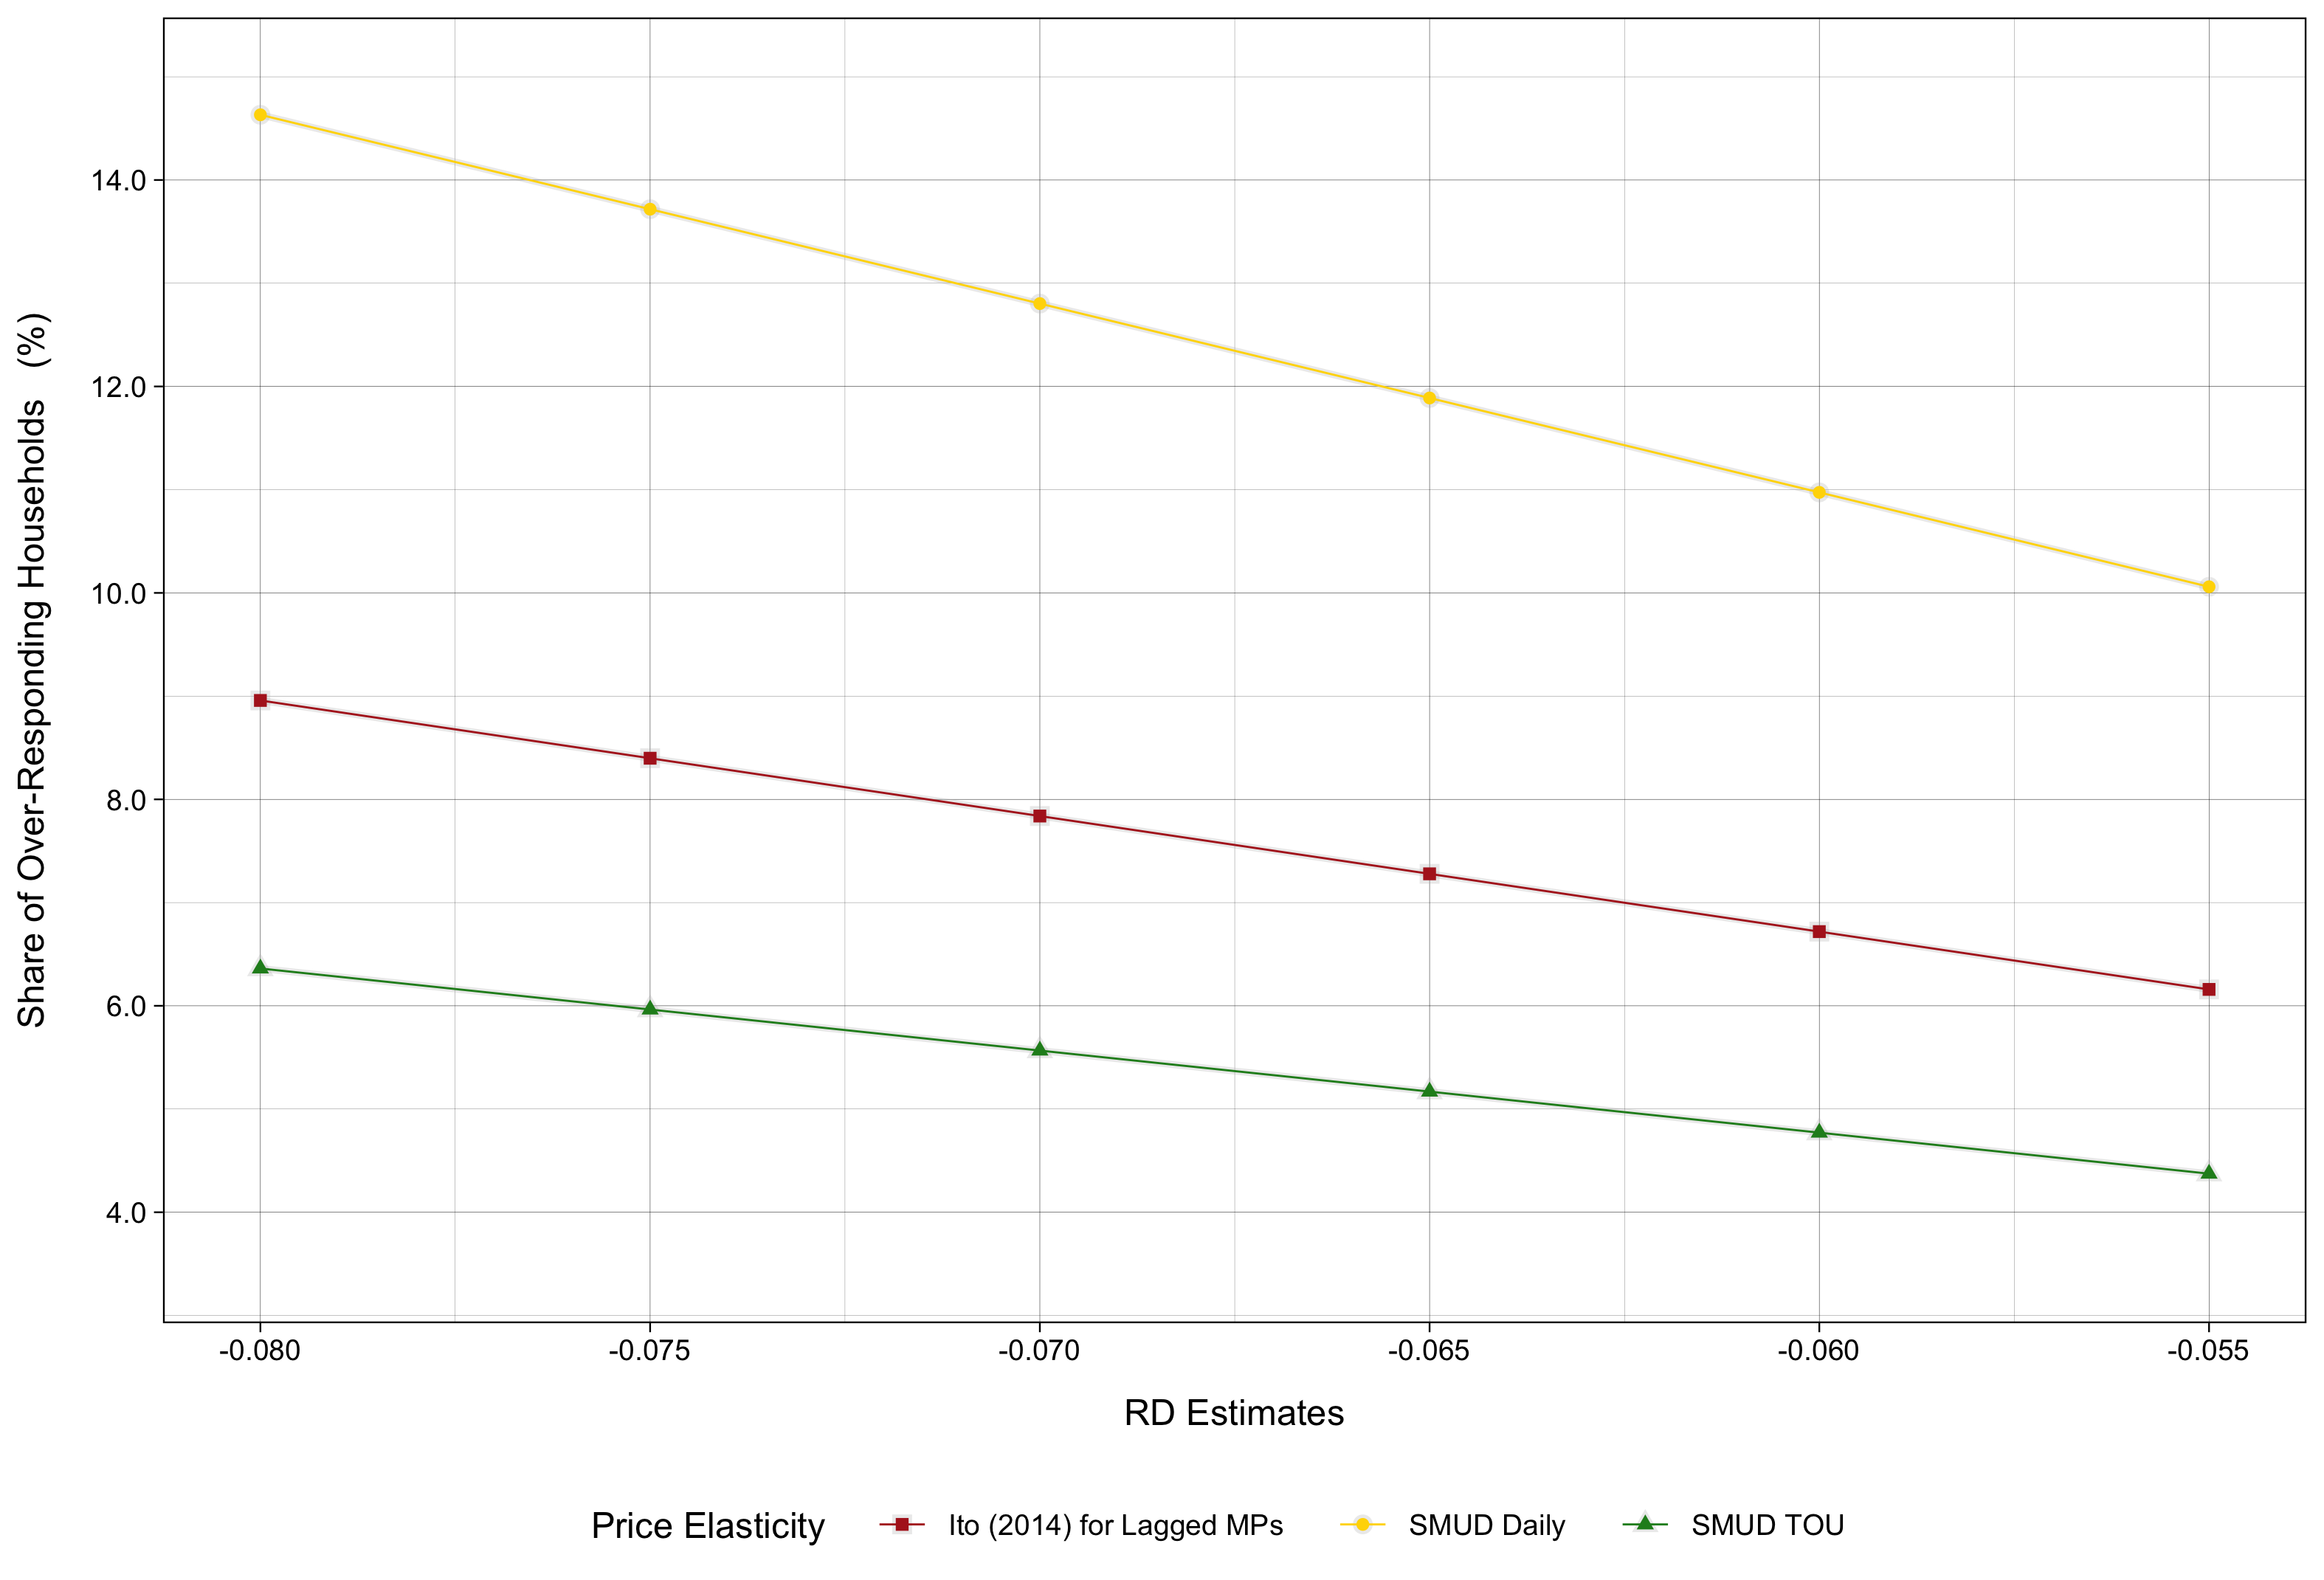
\includegraphics[scale = 0.143]{02_Chapter-1/00A_Figures/Figure_Share-of-Over-Responding-Households_RSGH.png}
        \caption{The Share of Over-Responding Households}
        \caption*{
            {\small
            \textit{Note}: 
            This figure shows, for different price elasticities of household electricity consumption, how the share of over-responding households varies with the value of the RD estimates. Two price elasticities for SMUD residential customers are in \cite{SmartPricing-Options-Final-Evaluation_SMUD_2014}, whereas the remaining price elasticity, estimated from PG\&E residential customers' billing data, is from \cite{Do-Consumers-Respond-to-Marginal-or-Average-Price?-Evidence-from-Nonlinear-Electricity-Pricing_2014_(Ito)}. See the text for details. 
        }}
        \label{Figure:Share-of-Over-Responding-Households_RSGH}
    \end{figure}
}
Inspired by \cite{Misunderstanding-Nonlinear-Prices_2020_(Shaffer)}, the estimates could be interpreted differently. The paper finds that a subgroup of less than 10\% of households, which applies the marginal price to all consumption, was driving the seemingly overall response, in which the primary response to the average price is masked. If this is also true in my setting, then the measured decrease in household electricity consumption would be attributed to a subset of my sample. Suppose that there are two distinct types of SMUD residential customers: households over-responding to the lagged marginal price and those not responding to it.\footnote{Here, I do not consider the type of households that respond to the average price because the change in the lagged marginal price at the threshold does not accompany any discontinuous change in the average price.} My back-of-the-envelope calculation suggests that about 11\% of over-responders produce the estimated treatment effect.\footnote{To obtain the proportion of over-responding households, I exploit the following values: 1) the daily price elasticity for default non-EAPR customers (i.e., $-0.030$), which is presented in \textit{Section 7.2 Price Elasticity Estimates} of \cite{SmartPricing-Options-Final-Evaluation_SMUD_2014}; and 2) the treatment effect, estimated with the value of bandwidth 10\%, for households selecting the RSGH rate plan (i.e., $-0.060$), which is given in Table \ref{Table:Robustness-Checks_BWs_RSGH}.} The share of over-responding households is obtained from the following steps: 1) computing the price elasticity of household electricity consumption by using the estimated treatment effect (i.e., the measured reduction in households' average daily electricity consumption), the average daily electricity consumption, the size of the price jump at the lower base usage quantity, and the average price at the cutoff point; and then 2) for a given price elasticity, which is available from other papers or reports, estimating how much households would have to respond to the lagged marginal price to obtain the price elasticity implied by my RD estimate. Moreover, for this computation, I exploit billing records only from non-electric-heating households (i.e., households choosing the RSGH rate plan.) Interestingly, my calculation, which indicates the reduction in electricity consumption by a subset of households in my sample, parallels the finding in the paper. Figure \ref{Figure:Share-of-Over-Responding-Households_RSGH} visualizes, for different price elasticities of residential electricity consumption, how the proportion of over-responding households varies with the magnitude of the RD estimates identified.  
